% One Britannica scan as extracted by Nemotron Parse 3.5. Filled by src/nemotron_challenge/stages/latex.py.
% The TITLE, BODY and SOURCE markers (each wrapped in two percent signs) are replaced. Compile with XeTeX (tectonic).
\documentclass[10pt]{article}
\usepackage[a4paper,margin=18mm]{geometry}
\usepackage{fontspec}
\usepackage{multicol}
\usepackage{graphicx}
\usepackage[hidelinks]{hyperref}
\setlength{\parindent}{0pt}
\setlength{\parskip}{4pt}
\setlength{\columnsep}{8mm}
\begin{document}
\section*{Historical source: scan row 2209}
\begin{center}
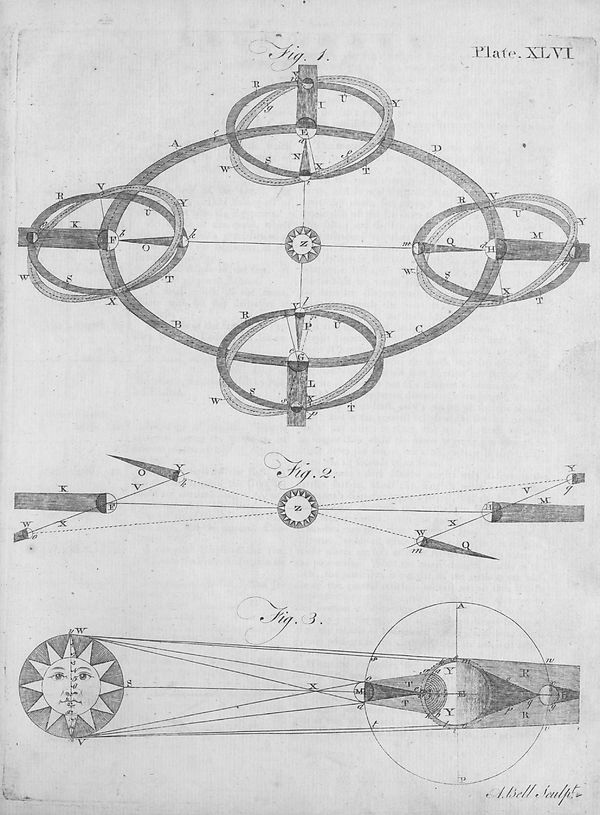
\includegraphics[width=\linewidth,height=0.4\textheight,keepaspectratio]{../crops/e2209-01.png}
\par{\small \textit{Plate:} Plate. XLVI}
\end{center}
\section*{Source record}
\begin{itemize}
\item Page ID: \texttt{britannica:309f765b1ecc83e0a7f7762e44b4a927a7555443:train:2209}
\item Scan: \texttt{page-2209-1ee9bc409f67.jpg}, 600 x 815 px
\item Image SHA-256: \texttt{\small 1ee9bc409f6798b0e4f4e45d63d75caae5197059df72701387ee24385cbff28e}
\item Extraction: \texttt{nvidia/nemotron-3.5-parse}, raw reply \texttt{artifacts/extract/raw/2209.json}
\item Text is Parse OCR output, normalized (long s as s, line-end hyphens joined). It is not corrected by hand.
\end{itemize}
\end{document}
